\documentclass[11pt,a4paper]{article}
\usepackage{pgfplots}
\pgfplotsset{compat=1.18}
% =========================
% Packages
% =========================
\usepackage[margin=1in]{geometry}
\usepackage{amsmath, amssymb, amsthm}
\usepackage{mathtools}
\usepackage{physics}
\usepackage{bm}
\usepackage{mathrsfs}

\usepackage{enumitem}
\usepackage{hyperref}
\usepackage{xcolor}
\usepackage{fancyhdr}
\usepackage{setspace}
\usepackage{graphicx}

% =========================
% Page Style
% =========================
\pagestyle{fancy}
\fancyhf{}
\lhead{\textsc{Lecture Notes}}
\rhead{\textsc{MAT211}}
\cfoot{\thepage}

\setstretch{1.15}

% =========================
% Custom Colors
% =========================
\definecolor{theoremcolor}{RGB}{0,0,120}
\definecolor{definitioncolor}{RGB}{0,90,0}
\definecolor{examplecolor}{RGB}{120,0,0}

% =========================
% Theorem Environments
% =========================
\theoremstyle{definition}
\newtheorem{definition}{Definition}[section]
\newtheorem{example}[definition]{Example}
\newtheorem{remark}[definition]{Remark}
\newtheorem{problem}[definition]{Problem}

\theoremstyle{plain}
\newtheorem{theorem}[definition]{Theorem}
\newtheorem{proposition}[definition]{Proposition}
\newtheorem{lemma}[definition]{Lemma}
\newtheorem{corollary}[definition]{Corollary}

% =========================
% Custom Commands
% =========================
\newcommand{\R}{\mathbb{R}}
\newcommand{\C}{\mathbb{C}}
\newcommand{\N}{\mathbb{N}}
\newcommand{\Z}{\mathbb{Z}}
\newcommand{\Q}{\mathbb{Q}}

\newcommand{\eps}{\varepsilon}

% =========================
% Title Info
% =========================
\title{\textbf{MAT211: Calculus-II}\\
\large Lecture Notes}
\author{Instructor: Emon Hossain}
\date{\today}

% =========================
% Document
% =========================
\begin{document}

\maketitle
\vspace{-1em}

\tableofcontents
\newpage

% =========================
% Lecture Starts
% =========================
\section{Lecture-01}

\textbf{Question:} what did we mean by the derivative $f'(a)$?\\
\textbf{Answer:} Let \textcolor{red}{$U$ be an open subset} of $\mathbb R$ and $f:U\rightarrow \mathbb R$ a function. Then $f$ is differentiable at $a$, with derivative $m$, if and only if
\begin{equation}
\label{diff_1}
    \lim_{h\rightarrow 0}\frac{1}{h}\left( \underbrace{f(a+h)-f(a)}_{\Delta f} - \underbrace{mh}_{(*)} \right)=0
\end{equation}
$(*):$ linear function of $\Delta x=h$.\\
\textbf{Question:} Why impose the domain $U$ that needs to be an open set?\\ 
\textbf{Answer:} Write the answer.\\
The function $mh$ that multiplies $h$ by the derivative $m$ is thus a linear function of the change in $x$. This definition emphasizes the idea that a function $f$ is differentiable at a point $a$ if the increment $\Delta f$ to the function is well approximated by a linear function of the increment $h$ to the variable, this linear function is $f'(a)h$. Let's see how we can confirm that:\\
Suppose $f(x)$ is our desired function and we want to approximate the function in the neighborhood at $x=a$. For this purpose, we will draw several straight lines through the point $(a,f(a))$ and see which line approximates the function best. Here, the best means, the linear line should approximate the function well at $x=a+h$. Suppose the slope of that linear function is $m$.   
\begin{center}
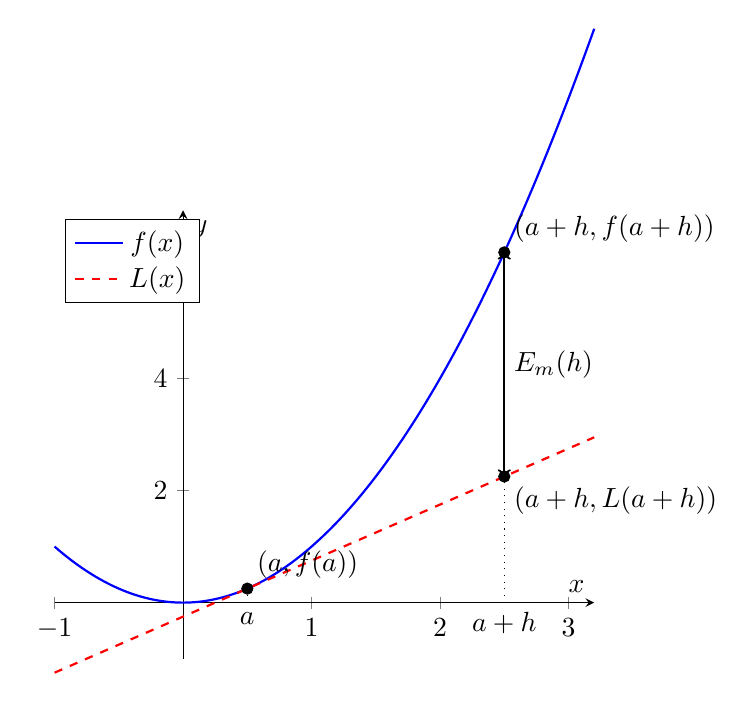
\begin{tikzpicture}
\begin{axis}[
    axis lines = middle,
    xlabel={$x$},
    ylabel={$y$},
    xmin=-1, xmax=3.2,
    ymin=-1, ymax=7,
    samples=200,
    domain=-1:3.2,
    legend style={at={(0.02,0.98)},anchor=north west},
    clip=false
]

% ---- Choose a function (example) ----
% f(x)=x^2, f'(x)=2x
\addplot[blue, thick] {x^2};
\addlegendentry{$f(x)$}

% ---- Parameters a and h ----
\def\a{0.5}
\def\h{2}

% Values at a, and at a+h
\pgfmathsetmacro{\fa}{(\a)^2}
\pgfmathsetmacro{\apH}{\a+\h}
\pgfmathsetmacro{\fapH}{(\apH)^2}

% Tangent line at x=a:  y = f(a)+f'(a)(x-a)  ;  f'(a)=2a
\addplot[red, thick, dashed] {2*\a*(x-\a)+\fa};
\addlegendentry{$L(x)$}

% Tangent prediction at x=a+h:  L(a+h)=f(a)+f'(a)h
\pgfmathsetmacro{\LapH}{\fa + 2*\a*\h}

% ---- Mark key points ----
\addplot[black, mark=*] coordinates {(\a,\fa)};
\node[above right] at (axis cs:\a,\fa) {$(a,f(a))$};

\addplot[black, mark=*] coordinates {(\apH,\fapH)};
\node[above right] at (axis cs:\apH,\fapH) {$(a+h,f(a+h))$};

\addplot[black, mark=*] coordinates {(\apH,\LapH)};
\node[below right] at (axis cs:\apH,\LapH) {$(a+h,L(a+h))$};

% Vertical reference lines at a and a+h
\addplot[dotted] coordinates {(\a,0) (\a,\fa)};
\node[below] at (axis cs:\a,0) {$a$};

\addplot[dotted] coordinates {(\apH,0) (\apH,\fapH)};
\node[below] at (axis cs:\apH,0) {$a+h$};

% ---- Error: E(h) = f(a+h) - L(a+h) ----
\draw[<->, thick]
  (axis cs:\apH,\LapH) -- (axis cs:\apH,\fapH);

\node[right] at (axis cs:\apH, {(\LapH+\fapH)/2})
{$E_m(h)$};
\end{axis}
\end{tikzpicture}
\end{center}
Then, 
\begin{align*}
    \frac{L(a+h)-L(a)}{a+h-a}&=m\\
    \frac{L(a+h)-f(a)}{h}&=m\\
    L(a+h)&=f(a)+mh
\end{align*}
Now, we want to minimize the error, $E_m(h)=f(a+h)-L(a+h)$. Hence, we need to find the optimal value for $m$, for which: 
\begin{align*}
    \frac{E_m(h)}{h}&\rightarrow 0
\end{align*}
$$
\boxed{\text{optimal }m\iff\lim_{h\rightarrow0}\frac{E_m(h)}{h}=0}
$$
A simple computation show that, 
\begin{align*}
    \lim_{h\rightarrow0}\frac{E_m(h)}{h}=\lim_{h\rightarrow0}\frac{f(a+h)-f(a)-mh}{h}=0
\end{align*}
which is the desired condition \ref{diff_1}, we showed in the definition.  


\newpage
\section{Lecture-02}

\begin{definition}[Euclidean Vector Space]
	A Euclidean vector space is a finite-dimensional inner product space over $\R$.
\end{definition}

\begin{definition}[Inner product space]
	An inner product space is a vector space $V$ over the field $F$ together with an inner product, that is, a map
	\[ \langle \cdot,\cdot \rangle : V \times V \to F\]
	that satisfies the following three properties for all vectors $x,y,z \in V$ and all scalars $a,b \in F$.
	\begin{enumerate}
		\item (Symmetry) $\langle x,y \rangle = \langle y,x \rangle$.
		\item (Linearity in the first argument)  $\langle ax + by,z \rangle = a \langle x,z \rangle + b \langle y,z \rangle$.

		\item (Positive-definiteness) If $x \neq 0$ then,  $\langle x,x \rangle  > 0$.
	\end{enumerate}
\end{definition}

\begin{example}
	Verify that the dot product function $\langle \cdot, \cdot \rangle : \R \times \R \to \R$ is an inner product.

	To verify this we must prove the three conditions shown above. Let $u = (a,b)$ and  $v = (c,d)$. Then,
	\begin{enumerate}
		\item $\langle u, v \rangle = ac + bd = ca + db = \langle v,u \rangle.$
		\item Let $a,b \in \R$ and $u,v,w \in \R^2$ with $u = (u_1,u_2), v = (v_1,v_2), w = (w_1,w_2)$. Then

	\end{enumerate}
	\begin{align*}
		\langle au + bv, w \rangle & = (au_1 + bv_1) w_1 + (au_2+bv_2) w_2            \\
		                           & = au_1w_1 + bv_1w_1 + au_2w_2 + bv_2w_2          \\
		                           & = a(u_1w_1 + u_2w_2) + b(v_1w_1 + v_2w_2)        \\
		                           & = a \langle u,w \rangle + b \langle v,w \rangle.
	\end{align*}
	\begin{enumerate}
		\item[3.] For any $u = (u_1,u_2)$,
		      \[ \langle u, u \rangle = {u_1}^2 + {u_2}^2.\]
		      Since squares of non-zero numbers are positive, we have  ${u_1}^2 >0, {u_2}^2 > 0$ and therefore,  $\langle u,u \rangle > 0$.
	\end{enumerate}
\end{example}

\begin{definition}[Informal]
	Define \textbf{norm} of a vector $x \in V$ as
	\[ || x || = \sqrt{\langle x,x \rangle}.\]
\end{definition}

\begin{definition}[Metric Space]
	A metric space is an ordered pair $(M,d)$ where $M$ is a set and $d$ is a \textbf{metric} (distance) on $M$, i.e., a function
	\[d : M \times M \to \R\]
	satisfying the following axioms for all points $x,y,z \in M$ :
	\begin{enumerate}
		\item $d(x,y) \geq 0$;
		\item $d(x,y) = 0 \iff x = y$ ;
		\item $d(x,y) = d(y,x)$.
		\item $d(x,z) \leq d(x,y) + d(y,z)$.
	\end{enumerate}
\end{definition}

\begin{example}[Tax-cab Metric]
	In $\R^2$, the taxi-cab distance between $p=(p_1,p_2)$ and $q=(q_1,q_2)$ is
	$|q_1 - p_1| + |q_2 - p_2|$. It is easy to verify that this is a metric.
\end{example}

\begin{definition}[Open ball]
	For any $x \in \R^n$ and any $r > 0$, the \textbf{open ball} of radius $r$ around $x$ is the subset
	\[B_r(x) = \{y \in \R^n \mid |x-y| < r\}.\]
\end{definition}

\begin{center}
	\includegraphics[scale=0.18]{Lectures/images/open-set.jpg}
\end{center}

\begin{definition}[Open sets of $\R^n$ ]
	A subset $U \subseteq \R^n$ is open if for every point $x \in U$, there exists $r > 0$ such that the open ball $B_r(x)$ is contained in $U$.
\end{definition}

\begin{example}
	We prove that the Cartesian product \((a_1,b_1)\times(a_2,b_2)\) of two open intervals in \(\mathbb{R}\) is an open set in \(\mathbb{R}^2\) with the standard Euclidean topology.

	\begin{proof}
		Let \(d\) denote the Euclidean metric on \(\mathbb{R}^2\):
		\[
			d\big((x_1,y_1),(x_2,y_2)\big)=\sqrt{(x_1-x_2)^2+(y_1-y_2)^2}.
		\]
		Take an arbitrary point \(p=(x,y)\in (a_1,b_1)\times(a_2,b_2)\). Then
		\[
			a_1 < x < b_1,\qquad a_2 < y < b_2.
		\]
		Define the four positive distances to the endpoints:
		\[
			d_1 = x - a_1,\quad d_2 = b_1 - x,\quad d_3 = y - a_2,\quad d_4 = b_2 - y.
		\]
		Let
		\[
			r = \min\{d_1,d_2,d_3,d_4\}>0.
		\]
		We claim that the open ball \(B(p,r)=\{q\in\mathbb{R}^2 : d(p,q)<r\}\) is contained in \((a_1,b_1)\times(a_2,b_2)\).

		Indeed, take any point \(q=(u,v)\in B(p,r)\). Then
		\[
			|u-x|\le d(p,q)<r,\qquad |v-y|\le d(p,q)<r.
		\]
		Hence
		\[
			x-r < u < x+r,\qquad y-r < v < y+r.
		\]
		Because \(r\le x-a_1\) and \(r\le b_1-x\), we have
		\[
			a_1 \le x-r < u < x+r \le b_1,
		\]
		so \(u\in(a_1,b_1)\). Similarly, \(r\le y-a_2\) and \(r\le b_2-y\) imply
		\[
			a_2 \le y-r < v < y+r \le b_2,
		\]
		so \(v\in(a_2,b_2)\). Consequently \(q=(u,v)\in(a_1,b_1)\times(a_2,b_2)\).

		Thus every point of the product has an open neighbourhood (an open ball) contained in the product. By definition, \((a_1,b_1)\times(a_2,b_2)\) is open in \(\mathbb{R}^2\).
	\end{proof}
\end{example}

\begin{definition}[Closed set]
	A closed set $A$ is defined by its ability to contain all of its limit points, meaning if a sequence of points $\{x_n\}$ within $A$ converges to a limit $x$, then that limit $x$ must also be in $A$.
\end{definition}

\begin{definition}[Sequence]
	A sequence is a function whose domain is $\N$.
\end{definition}

% \begin{definition}[Metric Space]
% Let $X$ be a set. A function
% \[
% d : X \times X \to \R
% \]
% is called a \emph{metric} if for all $x,y,z \in X$:
% \begin{enumerate}[label=(\roman*)]
%     \item $d(x,y) \ge 0$ and $d(x,y)=0$ iff $x=y$,
%     \item $d(x,y)=d(y,x)$,
%     \item $d(x,z) \le d(x,y)+d(y,z)$.
% \end{enumerate}
% \end{definition}

% \begin{example}
% The function
% \[
% d(x,y) = |x-y|
% \]
% defines a metric on $\R$.
% \end{example}

% \section{Main Results}

% \begin{theorem}[Triangle Inequality in $\R^n$]
% For all $x,y \in \R^n$,
% \[
% \|x+y\| \le \|x\| + \|y\|.
% \]
% \end{theorem}

% \begin{proof}
% Let $x,y \in \R^n$. Using the dot product,
% \[
% \|x+y\|^2 = \|x\|^2 + \|y\|^2 + 2\langle x,y\rangle.
% \]
% By the Cauchy–Schwarz inequality,
% \[
% \langle x,y\rangle \le \|x\|\,\|y\|.
% \]
% Hence,
% \[
% \|x+y\|^2 \le (\|x\|+\|y\|)^2.
% \]
% Taking square roots gives the result.
% \end{proof}

% \section{Worked Problems}

% \begin{problem}
% Show that $d(x,y)=\min\{1,|x-y|\}$ defines a metric on $\R$.
% \end{problem}

% \begin{proof}
% Non-negativity and symmetry are immediate.  
% For the triangle inequality, observe that
% \[
% |x-z| \le |x-y| + |y-z|
% \]
% and apply the monotonicity of $\min\{1,t\}$.
% \end{proof}

% \section{Remarks and Further Discussion}

% \begin{remark}
% Different choices of metrics can induce the same topology but lead to different geometric properties.
% \end{remark}

% =========================
% End
% =========================
\end{document}
